\section{Numerical validations}
\label{ap:validation}
The \texttt{Basilisk} code has been validated numerous times in previous numerical studies. 
Especially, we can cite the recent studies of \citet{innocenti2020direct} and \citet{hidman2023assessing} which both performed DNS of rising suspensions of bubbles. 
Nevertheless, in this work we investigate specific statistical distributions,
and we make use of a multi-VoF method to avoid droplets coalescence, therefore a meticulous validation of the DNS is in order. 
We start by presenting a brief comparison with the reference DNS of \citet{esmaeeli1999direct}. 
Afterward we present a study focusing on the interface kinematics where we compare our DNS with the experimental results of \citet{mohamed2003drop} to show that the multi-VoF method indeed captures the physics of two colliding interfaces without resolving the flow within the separating film. 
Once the mesh and the physics are validated, a study on the convergence of the statistics is presented. 

\subsection{Ordered array of buoyant bubbles}

From our knowledge, no simulations nor experimental results have been carried out for rising buoyant viscous droplets. 
Therefore, we reproduced instead the ordered array simulation of \citet{esmaeeli1999direct} with \texttt{Basilisk} to validate the mesh resolution of our DNS.  
It consists in a 3-D buoyant ordered rising array of bubbles. 
In our notation the flow parameters of the simulation read 
\begin{align*}
    \lambda = 10,
    && \zeta = 10,
    && Bo = 1.8,
    && Ga = 28.37,
    && \phi = 0.125.
\end{align*}
\begin{figure}[h!]
    \centering
    \includegraphics[height = 0.3\textwidth]{image/VALIDATION2.0/Loisy/Re.pdf}
    \caption{Time evolution of the Reynolds number based on the instantaneous volume averaged drift velocity, $Re_d(t) = \rho_fU _dd /\mu_f$, with $U_d(t)$ the drift velocity defined as $U_d = |\textbf{u}_d - \textbf{u}|$ with $\phi = 0.1256$, $\zeta =\mu_r =10$ and $Ga = 29.9$. $\textbf{u}_d$ and $\textbf{u}$ represent the volume-averaged velocities of the dispersed phase and the bulk, respectively, at time $t$.}
    %$\textbf{u}_d$ and $\textbf{u}$ are the average of the dispersed phase velocity and bulk velocity at time $t$ respectively.}
    \label{fig:ordered_array}
\end{figure}
\ref{fig:ordered_array} displays our numerical simulation against the original result of \citet{esmaeeli1999direct}.
We observe very good agreements between both studies for all mesh resolutions.
Additionally, we displayed the results of \citet{innocenti2020direct} for $d/\Delta = 20$ to point out a divergence with our results at the same mesh resolution.  
Both our simulations and the one of \citet{innocenti2020direct} have been carried out with the  \texttt{Basilisk} code. 
The cause of this difference is in fact due to a different method of interpolation used for the viscosity coefficient $\mu$. 
We used an arithmetic mean whereas \citet{innocenti2020direct} used an 
harmonic mean.
As a matter of fact in this regime the arithmetic mean, which will be used in this work, permits us to reach a faster convergence. 
Overall these results indicate that the criterion $d/\Delta = 20$ seems sufficient.%, which is consistent with the aforementioned studies.


\subsection{Drop impact on a liquid-liquid interface}

In this section we investigate in more detail the physics behind the multi-VoF method. 
We need to verify if we accurately capture the physics of the droplets interfaces despite the fact that we do not resolve accurately the film between two droplets. 
Following \citet{balcazar2015multiple} we reproduced the experiment of drop impact on a liquid–liquid interface carried by \citet{mohamed2003drop} but with the \texttt{Basilisk} code. 
This experiment consists in letting a drop fall into a pool of the same fluid as the drop. 
All along the experiment the interfaces of the droplets and the pool are tracked. 
In our notation the dimensionless parameters read 
\begin{align*}
    Ga = 71.02 
    && Bo = 6.40
    && \lambda = 0.33
    && \zeta = 1.189
\end{align*}
Following \citet{mohamed2003drop} we defined the dimensionless time $t / t_i = t U_i(t) /d$ where $U_i(t)$ is droplet velocity at $t<0$ and where $t=0$ is the time of impact. 
Regarding the geometry of the problem we sketched in \ref{fig:schemeLong} the initial position of the droplet in the computational domain.
Additionally, we display on \ref{fig:schemeLong} a snapshot of the numerical domain were we see the drop colliding the pool interface.
The drop and the pool do not merge since we use the multi-VoF method. 
Note that in the experiment the drop does not merge with the pool either.
This enables us to represent with the DNS a physical situation where the interfaces do not coalesce, but where we use a grid resolution of $d/\Delta = 20$ which is of course not sufficient to resolve the flow inside the film. 
\begin{figure}[h!]
    \centering
    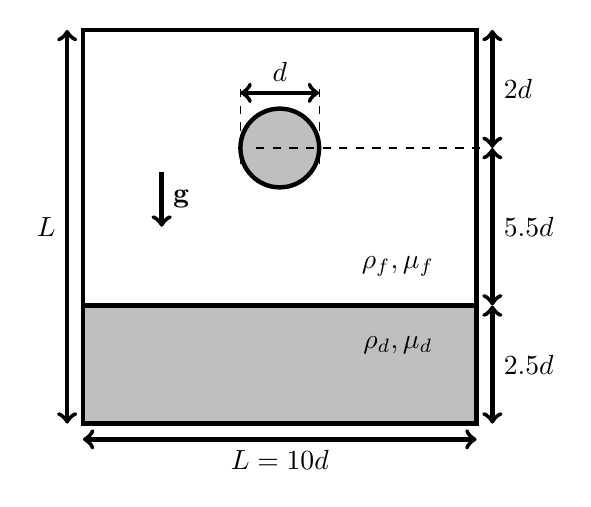
\begin{tikzpicture}[ultra thick]
        \draw (0,0) rectangle (5,5);
        \draw[fill=gray!50] (0,0) rectangle (5,1.5);
        \draw[fill=gray!50] (2.5,3.5) circle (0.5);
        \draw[<->](0,-0.2) --++ (5,0)node[midway,below]{$L  = 10 d$};
        \draw[<->](-0.2,0) --++ (0,5)node[midway,left]{$L$};
        \draw[<->](5.2,0) --++ (0,1.5)node[midway,right]{$2.5 d$};
        \draw[<->](5.2,1.5) --++ (0,2)node[midway,right]{$5.5 d$};
        \draw[<->](5.2,3.5) --++ (0,1.5)node[midway,right]{$ 2d$};
        \draw[dashed,thin](2.2,3.5) --++ (2.9,0);
        \draw[dashed,thin](2.2,3.5) --++ (2.9,0);
        \draw[->](1,3.2) --++ (0,-0.7)node[midway,right]{$\textbf{g}$};
        \draw[<->](2,4.2) --++ (1,0)node[midway,above]{$d$};
        \draw[thin,dashed](2,3.3) --++ (0,1);
        \draw[thin,dashed](3,3.3) --++ (0,1);
        \node (a) at (4,2){$\rho_f, \mu_f$};
        \node (a) at (4,1){$\rho_d, \mu_d$};
    \end{tikzpicture}
    \includegraphics[height = 0.4\textwidth]{image/VALIDATION2.0/Longmire/IMG/image-079.png}
    \caption{(left) Sketch of the computational set up at the initial time. 
    (right) Snapshot of the computational domain after the collision, with the pool interface represented in gray.
    The background color represents the velocity field magnitude, which is undisturbed, indicating a large enough domain. }
    \label{fig:schemeLong}
\end{figure}
\begin{figure}[h!]
    \centering
    \includegraphics[height = 0.3\textwidth]{image/VALIDATION2.0/Longmire/Re.pdf}
    \includegraphics[height = 0.3\textwidth]{image/VALIDATION2.0/Longmire/Dist.pdf}
    \caption{(left) Time evolution of the Reynolds number based on the droplet velocity, $Re(t) = \rho_fU d /\mu_f$ as a function of the dimensionless time, (+) numerical results of  \citet{balcazar2015multiple} (right)  position of the interfaces, ($\bullet$) top droplet surface, ($+$) bottom droplet surface, (x) pool surface. (Symbols) Experimental results of \citet{mohamed2003drop} (solid line) present numerical simulations with $d/\Delta = 20$. }
    \label{fig:resultslong}
\end{figure}
\ref{fig:resultslong} represents the comparison between our results and the experiment of \citet{mohamed2003drop} (right) and the numerical simulation of \citet{balcazar2015multiple} (left). 
The time-dependent Reynolds number as well as the interfaces positions are shown to closely match both the numerical and experiential results. 
From the very good agreement we conclude that the kinematics are well-represented even during contact for a mesh resolution of $d/\Delta = 20$.

\subsection{Mesh independence and statistical convergence for random arrays of drops}

Even though the aforementioned studies carried validations of the \texttt{Basilisk} code for rising droplets or bubbles, almost all of them considered isolated droplets or bubbles as the only validation case. 
To the author's knowledge, to this date no published study has presented a mesh independence study for random arrays of droplets or bubbles of this scale. 
As particle interactions and higher \textit{Galileo} numbers may be more challenging to model, it is primordial to investigate the mesh independence of the DNS that are carried in this work. 
In this objective we performed a DNS of a random array of $N_b=125$ droplets, with the following parameters
\begin{align*}
    \lambda = 10,
    && \zeta = 1.11,
    && Bo = 0.2,
    && Ga = 100,
    && \phi = 0.1,
    && N_b =125,
\end{align*}
with mesh resolutions of $d/\Delta = 5,\; 10,\; 18,\; 37$. 
This set of parameters have been selected following these arguments :
A viscosity ratio $\lambda = 10$ induces more vorticity at the droplets interfaces in contrast with the $\lambda = 1$ cases. 
For high inertia regimes ($Ga = 100$) the boundary layers at the droplet interfaces require the fine grid to be resolved compared to the low inertia cases. 
At $\phi = 0.1$, numerous interactions of droplets are present, implying that the good modeling of the liquid films between interfaces becomes predominant on the overall hydrodynamic, this also requires a good mesh resolution. 
% Additionally, the lower \textit{Bond} number employed here ($Bo=0.2$ instead of $Bo =0.5$) requires a higher mesh quality as well. 
For these reasons, we suppose that this case might require the finest grid among all other cases presented in this study. 
Based on this remark we can assume that if this case is mesh independent, then all cases from \ref{tab:simulations} are equally validated. 

Let us first verify the independence of the drift velocity on the mesh resolution. 
\begin{figure}[h!]
    \centering
    \includegraphics[height = 0.3\textwidth]{image/HOMOGENEOUS_NEW/VAL/tr.pdf}
    \includegraphics[height = 0.3\textwidth]{image/HOMOGENEOUS_NEW/VAL/Re.pdf}
    \caption{
        (left) Running average of the trace of $\textbf{R}$ as a function of the dimensionless time $t \sqrt{d/g}$. 
        (right) Running average of the Reynolds number based on the instantaneous volume-averaged relative velocity, $Re(t) = \rho_f U d /\mu_f$, with $U(t) = |\textbf{u}_d - \textbf{u}_c|$ for $\phi = 0.1$, $Ga=100$ and $\lambda =10$. 
        $\textbf{u}_d$ and $\textbf{u}_c$ represent the volume-averaged velocities of the dispersed phase and the continuous phase, respectively, at the dimensionless time $t \sqrt{d/g}$.
        %$\textbf{u}_p$ and $\textbf{u}_f$ are the particle and fluid phase volume averaged velocity at time $t$.
        In the legend we display the value of the mesh resolution. 
    }
    \label{fig:Re}
\end{figure}
In \ref{fig:Re} we display the running-averaged drift velocity as a function of time, for four mesh resolutions. 
The results are not as independent of the mesh resolution as the ordered array validation presented above. 
Indeed, we observe a difference of the rising Reynolds number of about $5\%$ between the $d/\Delta = 18$ and $d/\Delta = 37$ cases which is notable.
We recall that this $5\%$ error will eventually be lower for all other cases. 
The good agreement between the case  $d/\Delta = 10$ and $d/\Delta = 18$ is partially fortuitous.


% In \ref{fig:Re} (right) we display the running-averaged drift velocity as a function of time, for five mesh resolutions. 
% The results are not as independent of the mesh resolution as the ordered array validation presented above. 
% Indeed, we observe a difference of the rising Reynolds number of about $ 3\%$ between the $d/\Delta = 25$ and $d/\Delta = 60$ cases which is notable.
% We recall that this $3\%$ error will eventually be lower for all other cases. 

Now, let us turn our attention to \ref{fig:Re} (left), where we display the running average of $\text tr(\textbf{R})/r_m^2$ for different mesh resolutions.  
This figure validates two important points. 
First, we notice that the average of $\text tr(\textbf{R})/r_m^2$ appears well-converged at large $t\sqrt{d/g}$. 
This indicates that we have gathered a sufficient number of statistics to obtain accurate results. 
Secondly, it is found that the four cases converge approximately to the same value at large  $t\sqrt{d/g}$, implying that this quantity is also mesh-independent. 

\subsection{ Domain size independence study}

As discussed in the main text, the length scale of the distance between the particle layers is of the same order as the domain size. 
This raises an important question: Is the observed microstructure a physical phenomenon, or merely an artifact of the domain's size?
To address this, we conducted a DNS of a random array of $N_b=800$ droplets with a domain size of $\mathcal{L}/d = 20$. With the following dimensionless parameters:
\begin{align*}
    \lambda = 1,
    && \zeta = 1.11,
    && Bo = 0.5,
    && Ga = 80,
    && \phi = 0.05. 
\end{align*}
Note that the \textit{Galileo} number and the \textit{Bond} number are slightly different than in the original set of DNS due to numerical constraints.
We expect that these changes are not significant, so that the comparison remains valuable.


In \ref{fig:Pnst_large_domain} we compare the distribution $P_\text{nst}$ from the current case with $N_b =800$ droplets to the dataset used in this study with $N_b = 125$ droplets.
A good agreement is observed between the two distributions, although slight differences are noticeable.
These differences could be due to the different \textit{Galileo} numbers used in the larger simulation.
Nevertheless, the anisotropic behavior of $P_\text{nst}$ appears to be preserved between these two DNS.   
\begin{figure}[h!]
    \centering
    \includegraphics[height=0.205\textwidth]{image/HOMOGENEOUS_NEW/Dist/Pnst_l_1_Ga_100_PHI_0_05.pdf}
    \includegraphics[height=0.205\textwidth]{image/HOMOGENEOUS_final/Dist/Pnst_l_1_Ga_80_PHI_0_05.pdf}
    \caption{Histogram of the normalized function $P_\text{nst}$ at high inertia $Ga = 100$.
    The color map represents the values of the nearest pair distribution function. %of $P_\text{nst}$.
    The origin corresponds to the position of the \textit{\textit{test particle}}.
    The dimensionless radial and azimuthal coordinates, $|\textbf{r}|/d$ and $\theta$, correspond to the nearest neighbor position.
    The vertical direction corresponds to the flow direction, which is also the axis of symmetry for $P_\text{nst}$.
    (left) Original DNS with $N_b =125$ droplets.
    (right) Reference DNS with $N_b = 800$ droplets.}
    \label{fig:Pnst_large_domain}
\end{figure}
To provide a qualitative visualization of the system behavior, we displayed in \ref{fig:images_deux} a snapshot from both DNS. 
\begin{figure}[h!]
    \centering
    \includegraphics[width=0.45\textwidth]{image/HOMOGENEOUS_NEW/P_PHI_5_l_10_Ga_100.png}
    \includegraphics[width=0.45\textwidth]{image/HOMOGENEOUS_final/Ga_80_phi_005_l_1.png}
 %    \includegraphics[width=0.45\textwidth]{image/HOMOGENEOUS_NEW/Ga_100_phi_005_l_10.png}
    \caption{Snapshot of a simulation at $t^* = 150$ for $\phi=0.05$.
    Color map : values of the vertical component of the velocity, field on the vertical plane defined by the equation $z=0$. 
    (left)  Tipical DNS used in this study  with $\lambda = 1$ and $N_b = 125$ droplets.
    (right) A larger DNS with same $\phi$ and  $\lambda$ but with $N_b = 800$ droplets.
    }
    \label{fig:images_deux}
\end{figure}
We can observe that the DNS with $N_b = 800$ droplets also exhibits layers and clusters of droplets, similar to the original simulation. 
At this stage, we have not delved into quantitative analysis to verify if the distance between layers is consistent across both sets of simulations. 

Overall, we conclude that the domain size used in this work, $\mathcal{L}/d = 10$, is sufficient. 
Indeed, The distribution $P_\text{nst}$ remains similar in the larger domain (with $\mathcal{L}/d = 20$), and the microstructure displays the same types of particle layers and clusters.